\documentclass[12pt]{article}\usepackage[]{graphicx}\usepackage[]{color}
%% maxwidth is the original width if it is less than linewidth
%% otherwise use linewidth (to make sure the graphics do not exceed the margin)
\makeatletter
\def\maxwidth{ %
  \ifdim\Gin@nat@width>\linewidth
    \linewidth
  \else
    \Gin@nat@width
  \fi
}
\makeatother

\definecolor{fgcolor}{rgb}{0.345, 0.345, 0.345}
\newcommand{\hlnum}[1]{\textcolor[rgb]{0.686,0.059,0.569}{#1}}%
\newcommand{\hlstr}[1]{\textcolor[rgb]{0.192,0.494,0.8}{#1}}%
\newcommand{\hlcom}[1]{\textcolor[rgb]{0.678,0.584,0.686}{\textit{#1}}}%
\newcommand{\hlopt}[1]{\textcolor[rgb]{0,0,0}{#1}}%
\newcommand{\hlstd}[1]{\textcolor[rgb]{0.345,0.345,0.345}{#1}}%
\newcommand{\hlkwa}[1]{\textcolor[rgb]{0.161,0.373,0.58}{\textbf{#1}}}%
\newcommand{\hlkwb}[1]{\textcolor[rgb]{0.69,0.353,0.396}{#1}}%
\newcommand{\hlkwc}[1]{\textcolor[rgb]{0.333,0.667,0.333}{#1}}%
\newcommand{\hlkwd}[1]{\textcolor[rgb]{0.737,0.353,0.396}{\textbf{#1}}}%

\usepackage{framed}
\makeatletter
\newenvironment{kframe}{%
 \def\at@end@of@kframe{}%
 \ifinner\ifhmode%
  \def\at@end@of@kframe{\end{minipage}}%
  \begin{minipage}{\columnwidth}%
 \fi\fi%
 \def\FrameCommand##1{\hskip\@totalleftmargin \hskip-\fboxsep
 \colorbox{shadecolor}{##1}\hskip-\fboxsep
     % There is no \\@totalrightmargin, so:
     \hskip-\linewidth \hskip-\@totalleftmargin \hskip\columnwidth}%
 \MakeFramed {\advance\hsize-\width
   \@totalleftmargin\z@ \linewidth\hsize
   \@setminipage}}%
 {\par\unskip\endMakeFramed%
 \at@end@of@kframe}
\makeatother

\definecolor{shadecolor}{rgb}{.97, .97, .97}
\definecolor{messagecolor}{rgb}{0, 0, 0}
\definecolor{warningcolor}{rgb}{1, 0, 1}
\definecolor{errorcolor}{rgb}{1, 0, 0}
\newenvironment{knitrout}{}{} % an empty environment to be redefined in TeX

\usepackage{alltt}

\usepackage{amssymb,amsmath}
\usepackage{enumerate}
\usepackage{float}
\usepackage{verbatim}
\usepackage{setspace}
\usepackage{multicol}

%% LaTeX margin settings:
  \setlength{\textwidth}{7.0in}
\setlength{\textheight}{9in}
\setlength{\oddsidemargin}{-.5in}
\setlength{\evensidemargin}{0in}
\setlength{\topmargin}{-1.5cm}

%% tell knitr to use smaller font for code chunks
\def\fs{\footnotesize}
\def\R{{\sf R}}
\newcommand{\bfbeta}{\mbox{\boldmath $\beta$}}
\newcommand{\bfD}{\mbox{\boldmath $D$}}
\newcommand{\bfL}{\mbox{\boldmath $L$}}
\newcommand{\bfR}{\mbox{\boldmath $R$}}
\newcommand{\bfmu}{\mbox{\boldmath $\mu$}}
\newcommand{\bfv}{\mbox{\boldmath $V$}}
\newcommand{\bfX}{\mbox{\boldmath $X$}}
\newcommand{\bfy}{\mbox{\boldmath $y$}}
\newcommand{\bfb}{\mbox{\boldmath $b$}}
\newcommand{\ytil}{\mbox{$\tilde{y}$}}
\IfFileExists{upquote.sty}{\usepackage{upquote}}{}
\begin{document}


  
  
  \begin{center}
\large{Sampling: Midterm I} \\
Leslie Gains-Germain
\end{center}

\begin{doublespacing}

\begin{enumerate}

\item \begin{enumerate}

\item $\hat{t}_{SRS} = 5690$. See R code below.

\begin{knitrout}\footnotesize
\definecolor{shadecolor}{rgb}{0.969, 0.969, 0.969}\color{fgcolor}\begin{kframe}
\begin{alltt}
\hlstd{branches.srs} \hlkwb{<-} \hlkwd{c}\hlstd{(}\hlnum{50}\hlstd{,} \hlnum{67}\hlstd{,} \hlnum{53}\hlstd{,} \hlnum{63}\hlstd{,} \hlnum{64}\hlstd{,} \hlnum{64}\hlstd{,} \hlnum{41}\hlstd{,} \hlnum{38}\hlstd{,} \hlnum{35}\hlstd{,} \hlnum{41}\hlstd{,} \hlnum{40}\hlstd{,} \hlnum{39}\hlstd{,} \hlnum{42}\hlstd{,} \hlnum{75}\hlstd{,} \hlnum{88}\hlstd{,} \hlnum{71}\hlstd{,}
                  \hlnum{65}\hlstd{,} \hlnum{40}\hlstd{,} \hlnum{38}\hlstd{,} \hlnum{41}\hlstd{,} \hlnum{44}\hlstd{,} \hlnum{39}\hlstd{)}
\hlstd{that} \hlkwb{<-} \hlnum{110}\hlopt{*}\hlkwd{mean}\hlstd{(branches.srs)}
\hlstd{that}
\end{alltt}
\begin{verbatim}
## [1] 5690
\end{verbatim}
\end{kframe}
\end{knitrout}

\item $SE(\hat{t}_{SRS}) = \sqrt{\hat{V}(\hat{t}_{SRS})} = 81.6726$. See R code below.

\begin{knitrout}\footnotesize
\definecolor{shadecolor}{rgb}{0.969, 0.969, 0.969}\color{fgcolor}\begin{kframe}
\begin{alltt}
\hlstd{se.that} \hlkwb{<-} \hlkwd{sqrt}\hlstd{(}\hlnum{110} \hlopt{*} \hlstd{(}\hlnum{110}\hlopt{-}\hlnum{22}\hlstd{)} \hlopt{*} \hlkwd{sd}\hlstd{(branches.srs)} \hlopt{/} \hlnum{22}\hlstd{)}
\hlstd{se.that}
\end{alltt}
\begin{verbatim}
## [1] 81.7
\end{verbatim}
\end{kframe}
\end{knitrout}

\item A $95\%$ t-based confidence interval for $t_{SRS}$ is $(5520, 5860)$. See R code below. We are $95\%$ confident that the true total number of apples on all apple-bearing branches of these four trees is between $5520$ and $5860$ apples.

\begin{knitrout}\footnotesize
\definecolor{shadecolor}{rgb}{0.969, 0.969, 0.969}\color{fgcolor}\begin{kframe}
\begin{alltt}
\hlstd{tstar} \hlkwb{<-} \hlkwd{qt}\hlstd{(}\hlnum{0.975}\hlstd{,} \hlnum{21}\hlstd{)}
\hlstd{ci} \hlkwb{<-} \hlkwd{c}\hlstd{(that}\hlopt{-}\hlstd{tstar}\hlopt{*}\hlstd{se.that, that}\hlopt{+}\hlstd{tstar}\hlopt{*}\hlstd{se.that)}
\hlstd{ci}
\end{alltt}
\begin{verbatim}
## [1] 5520 5860
\end{verbatim}
\end{kframe}
\end{knitrout}

\item At a $5\%$ significance level, there is evidence that the true total number of apples on all apple-bearing branches of these four trees is different than $5500$ apples. We make this conclusion because the $95\%$ confidence interval for $t_{SRS}$ does not contain $5500$. 

\item $\hat{t}_{STR} = 5931.167$. See R code below. After rounding, I would estimate the population total $t_{STR}$ to be $5931$. 

\begin{knitrout}\footnotesize
\definecolor{shadecolor}{rgb}{0.969, 0.969, 0.969}\color{fgcolor}\begin{kframe}
\begin{alltt}
\hlstd{branches.str1} \hlkwb{<-} \hlkwd{c}\hlstd{(}\hlnum{53}\hlstd{,} \hlnum{64}\hlstd{,} \hlnum{61}\hlstd{,} \hlnum{58}\hlstd{,} \hlnum{66}\hlstd{,} \hlnum{57}\hlstd{)}
\hlstd{branches.str2} \hlkwb{<-} \hlkwd{c}\hlstd{(}\hlnum{46}\hlstd{,} \hlnum{40}\hlstd{,} \hlnum{38}\hlstd{,} \hlnum{42}\hlstd{,} \hlnum{40}\hlstd{,} \hlnum{39}\hlstd{)}
\hlstd{branches.str3} \hlkwb{<-} \hlkwd{c}\hlstd{(}\hlnum{66}\hlstd{,} \hlnum{80}\hlstd{,} \hlnum{74}\hlstd{,} \hlnum{89}\hlstd{)}
\hlstd{branches.str4} \hlkwb{<-} \hlkwd{c}\hlstd{(}\hlnum{40}\hlstd{,} \hlnum{38}\hlstd{,} \hlnum{39}\hlstd{,} \hlnum{33}\hlstd{,} \hlnum{44}\hlstd{,} \hlnum{35}\hlstd{)}
\hlstd{that.str} \hlkwb{<-} \hlnum{30}\hlopt{*}\hlkwd{mean}\hlstd{(branches.str1)}\hlopt{+}
            \hlnum{25}\hlopt{*}\hlkwd{mean}\hlstd{(branches.str2)}\hlopt{+}
            \hlnum{26}\hlopt{*}\hlkwd{mean}\hlstd{(branches.str3)}\hlopt{+}
            \hlnum{29}\hlopt{*}\hlkwd{mean}\hlstd{(branches.str4)}
\hlstd{that.str}
\end{alltt}
\begin{verbatim}
## [1] 5931
\end{verbatim}
\end{kframe}
\end{knitrout}

\item $SE(\hat{t}_{STR}) = \sqrt{\hat{V}(\hat{t}_{STR})} = 51.1827$. See R code below.

\begin{knitrout}\footnotesize
\definecolor{shadecolor}{rgb}{0.969, 0.969, 0.969}\color{fgcolor}\begin{kframe}
\begin{alltt}
\hlstd{se.that.str} \hlkwb{<-} \hlkwd{sqrt}\hlstd{(}\hlnum{30} \hlopt{*} \hlstd{(}\hlnum{30}\hlopt{-}\hlnum{6}\hlstd{)} \hlopt{*} \hlkwd{sd}\hlstd{(branches.str1)} \hlopt{/} \hlnum{6} \hlopt{+}
                      \hlnum{25} \hlopt{*} \hlstd{(}\hlnum{25}\hlopt{-}\hlnum{6}\hlstd{)} \hlopt{*} \hlkwd{sd}\hlstd{(branches.str2)} \hlopt{/} \hlnum{6} \hlopt{+}
                      \hlnum{26} \hlopt{*} \hlstd{(}\hlnum{26}\hlopt{-}\hlnum{4}\hlstd{)} \hlopt{*} \hlkwd{sd}\hlstd{(branches.str3)} \hlopt{/} \hlnum{4} \hlopt{+}
                      \hlnum{29} \hlopt{*} \hlstd{(}\hlnum{29}\hlopt{-}\hlnum{6}\hlstd{)} \hlopt{*} \hlkwd{sd}\hlstd{(branches.str4)} \hlopt{/} \hlnum{6}\hlstd{)}
\hlstd{se.that.str}
\end{alltt}
\begin{verbatim}
## [1] 51.2
\end{verbatim}
\end{kframe}
\end{knitrout}

\item A $95\%$ t-based confidence interval for $t_{STR}$ is $(5823, 6039)$. See R code below. We are $95\%$ confident that the true total number of apples on all apple-bearing branches of these four trees is between $5823$ and $6039$ apples.

\begin{knitrout}\footnotesize
\definecolor{shadecolor}{rgb}{0.969, 0.969, 0.969}\color{fgcolor}\begin{kframe}
\begin{alltt}
\hlstd{tstar.str} \hlkwb{<-} \hlkwd{qt}\hlstd{(}\hlnum{0.975}\hlstd{,} \hlnum{22}\hlopt{-}\hlnum{4}\hlstd{)}
\hlstd{ci.str} \hlkwb{<-} \hlkwd{c}\hlstd{(that.str}\hlopt{-}\hlstd{tstar.str}\hlopt{*}\hlstd{se.that.str, that.str}\hlopt{+}\hlstd{tstar.str}\hlopt{*}\hlstd{se.that.str)}
\hlstd{ci.str}
\end{alltt}
\begin{verbatim}
## [1] 5824 6039
\end{verbatim}
\end{kframe}
\end{knitrout}

\item At a $5\%$ significance level, there is evidence that the true total number of apples on all apple-bearing branches of these four trees is different than $5500$ apples. We make this conclusion because the $95\%$ confidence interval for $t_{STR}$ does not contain $5500$. 


\item Yes, stratification did seem to improve the estimation process because the variance of the total estimate found using the stratified SRS is less than the variance of the total estimate found using SRS. As a result, the confidence interval for $t_{STR}$ is narrower than the confidence interval for $t_{SRS}$.

\begin{knitrout}\footnotesize
\definecolor{shadecolor}{rgb}{0.969, 0.969, 0.969}\color{fgcolor}\begin{kframe}
\begin{alltt}
\hlstd{ci[}\hlnum{2}\hlstd{]}\hlopt{-}\hlstd{ci[}\hlnum{1}\hlstd{]}
\end{alltt}
\begin{verbatim}
## [1] 340
\end{verbatim}
\begin{alltt}
\hlstd{ci.str[}\hlnum{2}\hlstd{]}\hlopt{-}\hlstd{ci.str[}\hlnum{1}\hlstd{]}
\end{alltt}
\begin{verbatim}
## [1] 215
\end{verbatim}
\end{kframe}
\end{knitrout}

\end{enumerate}

\item \begin{enumerate}

\item A percentile-method $95\%$ confidence interval for $t_{SRS}$ is $(5045, 6380)$. A percentile-method $95\%$ confidence interval for $t_{STR}$ is $(5490, 5930)$. The output is shown below, and the R code for this section is shown in the R code appendix. 

\begin{singlespace}
\begin{knitrout}\footnotesize
\definecolor{shadecolor}{rgb}{0.969, 0.969, 0.969}\color{fgcolor}\begin{kframe}
\begin{verbatim}

ORDINARY NONPARAMETRIC BOOTSTRAP


Call:
boot(data = branches.srs, statistic = samptotal, R = Brep)


Bootstrap Statistics :
    original  bias    std. error
t1*     5690  -0.392         345
BOOTSTRAP CONFIDENCE INTERVAL CALCULATIONS
Based on 10000 bootstrap replicates

CALL : 
boot.ci(boot.out = boottotal, conf = 0.95)

Intervals : 
Level      Normal              Basic         
95%   (5014, 6367 )   (5000, 6335 )  

Level     Percentile            BCa          
95%   (5045, 6380 )   (5095, 6440 )  
Calculations and Intervals on Original Scale
\end{verbatim}
\end{kframe}
\end{knitrout}

\newpage

\begin{knitrout}\footnotesize
\definecolor{shadecolor}{rgb}{0.969, 0.969, 0.969}\color{fgcolor}\begin{kframe}
\begin{verbatim}

STRATIFIED BOOTSTRAP


Call:
boot(data = branches.str, statistic = samptotal, R = Brep, strata = stratum)


Bootstrap Statistics :
    original  bias    std. error
t1*     5710   -0.55         113
BOOTSTRAP CONFIDENCE INTERVAL CALCULATIONS
Based on 10000 bootstrap replicates

CALL : 
boot.ci(boot.out = boottotal, conf = 0.95)

Intervals : 
Level      Normal              Basic         
95%   (5489, 5932 )   (5490, 5930 )  

Level     Percentile            BCa          
95%   (5490, 5930 )   (5490, 5930 )  
Calculations and Intervals on Original Scale
\end{verbatim}
\end{kframe}
\end{knitrout}
\end{singlespace}

\item The bootstrap standard error of $\hat{t}_{SRS}$ is $345.1742$. A t-based $95\%$ confidence interval for $t_{SRS}$ is then $5690 \pm 2.0796*345.1742$, or $(4972, 6408)$ after rounding. The bootstrap standard error of $\hat{t}_{STR}$ is $113.0012$. A t-based $95\%$ confidence interval for $t_{STR}$ is then $5710 \pm 2.1009*113.0012$, or $(5472, 5948)$ after rounding. The code is shown below. Recall that \verb+that+ and \verb+that.str+ were defined in problem $1$. 

\begin{singlespace}
\begin{knitrout}\footnotesize
\definecolor{shadecolor}{rgb}{0.969, 0.969, 0.969}\color{fgcolor}\begin{kframe}
\begin{alltt}
\hlstd{ci.tbootsrs} \hlkwb{<-} \hlkwd{c}\hlstd{(}\hlnum{5690}\hlopt{-}\hlstd{tstar}\hlopt{*}\hlnum{345.1742}\hlstd{,} \hlnum{5690}\hlopt{+}\hlstd{tstar}\hlopt{*}\hlnum{345.1742}\hlstd{)}
\hlstd{ci.tbootstr} \hlkwb{<-} \hlkwd{c}\hlstd{(}\hlnum{5710}\hlopt{-}\hlstd{tstar.str}\hlopt{*}\hlnum{113.0012}\hlstd{,} \hlnum{5710}\hlopt{+}\hlstd{tstar.str}\hlopt{*}\hlnum{113.0012}\hlstd{)}
\end{alltt}
\end{kframe}
\end{knitrout}
\end{singlespace}

I'd like to point out that the estimate for $t_{STR}$ found by the \verb+boot+ function is different than the estimate for $t_{STR}$ we found in problem $1$ part $(e)$. The reason for this is because the \verb+boot+ function doesn't take into account the fact that we know the true stratum sizes in the population (it only knows the sample sizes that we took from each stratum). So, the program estimates the true stratum sizes based on the number of samples taken from each stratum. For example, $6$ apples were chosen from stratum $1$, so the program estimates the true stratum size to be $110*6/22 = 30$. The R code shown below explains how the \verb+boot+ function arrived at $5710$ as the estimate for $t_{STR}$ (rather than $5931$ found in part $1(e)$. I think it would be good to investigate how to incorporate the true stratum sizes, when they are known, into the \verb+boot+ function.

\begin{singlespace}
\begin{knitrout}\footnotesize
\definecolor{shadecolor}{rgb}{0.969, 0.969, 0.969}\color{fgcolor}\begin{kframe}
\begin{alltt}
\hlnum{110}\hlopt{*}\hlstd{(}\hlnum{6}\hlopt{*}\hlkwd{mean}\hlstd{(branches.str1)}\hlopt{+}\hlnum{6}\hlopt{*}\hlkwd{mean}\hlstd{(branches.str2)}\hlopt{+}\hlnum{4}\hlopt{*}\hlkwd{mean}\hlstd{(branches.str3)}\hlopt{+}
       \hlnum{6}\hlopt{*}\hlkwd{mean}\hlstd{(branches.str4))}\hlopt{/}\hlnum{22}
\end{alltt}
\begin{verbatim}
## [1] 5710
\end{verbatim}
\end{kframe}
\end{knitrout}
\end{singlespace}


\item Yes, I think the $t$-based confidence interval is a reasonable alternative to the percentile-based confidence interval because the bootstrap distributions of totals are mostly symmetric for both the SRS and the stratified SRS sampling plans (see below).  I also noticed that the intervals obtained via the percentile method are similar to the $t$-based intervals found above, which is another indication that the $t$-based interval is a reasonable alternative to the percentile-based confidence interval.

\begin{knitrout}\footnotesize
\definecolor{shadecolor}{rgb}{0.969, 0.969, 0.969}\color{fgcolor}
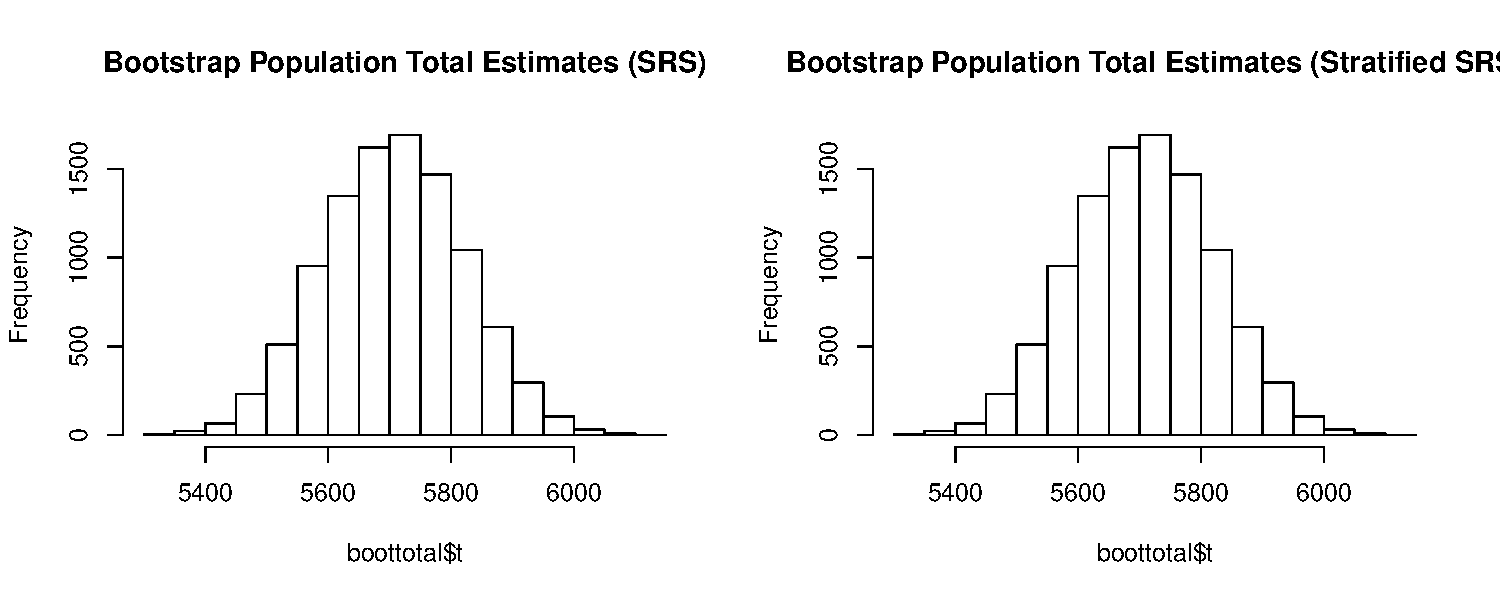
\includegraphics[width=\linewidth]{figure/hists-1} 

\end{knitrout}


\end{enumerate}

\item \begin{enumerate}
\item $\widehat{\bar{y}_U} = 12.9297$. See my work below.

\begin{singlespace}
\begin{knitrout}\footnotesize
\definecolor{shadecolor}{rgb}{0.969, 0.969, 0.969}\color{fgcolor}\begin{kframe}
\begin{alltt}
\hlstd{ybar1} \hlkwb{<-} \hlnum{175}\hlopt{/}\hlnum{25}
\hlstd{ybar2} \hlkwb{<-} \hlnum{400}\hlopt{/}\hlnum{25}
\hlstd{ybar3} \hlkwb{<-} \hlnum{375}\hlopt{/}\hlnum{16}
\hlstd{ybar4} \hlkwb{<-} \hlnum{176}\hlopt{/}\hlnum{16}
\hlstd{ybarhat} \hlkwb{<-} \hlstd{(}\hlnum{300}\hlopt{*}\hlstd{ybar1}\hlopt{+}\hlnum{300}\hlopt{*}\hlstd{ybar2}\hlopt{+}\hlnum{100}\hlopt{*}\hlstd{ybar3}\hlopt{+}\hlnum{100}\hlopt{*}\hlstd{ybar4)}\hlopt{/}\hlnum{800}
\hlstd{ybarhat}
\end{alltt}
\begin{verbatim}
## [1] 12.9
\end{verbatim}
\end{kframe}
\end{knitrout}
\end{singlespace}

\item The standard error of $\widehat{\bar{y}_U}$ is $1.2990$. See my work below.

\begin{singlespace}
\begin{knitrout}\footnotesize
\definecolor{shadecolor}{rgb}{0.969, 0.969, 0.969}\color{fgcolor}\begin{kframe}
\begin{alltt}
\hlstd{var.1} \hlkwb{<-} \hlnum{300}\hlopt{*}\hlstd{(}\hlnum{300}\hlopt{-}\hlnum{25}\hlstd{)}\hlopt{*}\hlnum{100}\hlopt{/}\hlnum{25}
\hlstd{var.2} \hlkwb{<-} \hlnum{300}\hlopt{*}\hlstd{(}\hlnum{300}\hlopt{-}\hlnum{25}\hlstd{)}\hlopt{*}\hlnum{100}\hlopt{/}\hlnum{25}
\hlstd{var.3} \hlkwb{<-} \hlnum{100}\hlopt{*}\hlstd{(}\hlnum{100}\hlopt{-}\hlnum{16}\hlstd{)}\hlopt{*}\hlnum{400}\hlopt{/}\hlnum{16}
\hlstd{var.4} \hlkwb{<-} \hlnum{100}\hlopt{*}\hlstd{(}\hlnum{100}\hlopt{-}\hlnum{16}\hlstd{)}\hlopt{*}\hlnum{400}\hlopt{/}\hlnum{16}
\hlstd{var.ybarhat} \hlkwb{<-} \hlnum{1}\hlopt{/}\hlstd{(}\hlnum{800}\hlopt{^}\hlnum{2}\hlstd{)}\hlopt{*}\hlstd{(var.1}\hlopt{+}\hlstd{var.2}\hlopt{+}\hlstd{var.3}\hlopt{+}\hlstd{var.4)}
\hlstd{se.ybarhat} \hlkwb{<-} \hlkwd{sqrt}\hlstd{(var.ybarhat)}
\hlstd{se.ybarhat}
\end{alltt}
\begin{verbatim}
## [1] 1.3
\end{verbatim}
\end{kframe}
\end{knitrout}
\end{singlespace}

\item A $95\%$ confidence interval for $\bar{y}_{U}$ is $(10.3435, 15.516)$. My work is shown below.

\begin{singlespace}
\begin{knitrout}\footnotesize
\definecolor{shadecolor}{rgb}{0.969, 0.969, 0.969}\color{fgcolor}\begin{kframe}
\begin{alltt}
\hlstd{tstar} \hlkwb{<-} \hlkwd{qt}\hlstd{(}\hlnum{0.975}\hlstd{,} \hlnum{82}\hlopt{-}\hlnum{4}\hlstd{)}
\hlstd{ci.ybar} \hlkwb{<-} \hlkwd{c}\hlstd{(ybarhat}\hlopt{-}\hlstd{tstar}\hlopt{*}\hlstd{se.ybarhat, ybarhat}\hlopt{+}\hlstd{tstar}\hlopt{*}\hlstd{se.ybarhat)}
\hlstd{ci.ybar}
\end{alltt}
\begin{verbatim}
## [1] 10.3 15.5
\end{verbatim}
\end{kframe}
\end{knitrout}
\end{singlespace}

\item If proportional allocation had been used, the sample sizes for strata $1$ and $2$ would have been $31$ ($300/800*82$). The sample sizes for strata $3$ and $4$ would have been $10$ ($100/800*82$). 

\item If optimum allocation had been used, the sample sizes for strata $1$ and $2$ would be $25$, and the sample sizes for strata $3$ and $4$ would be $16$. Clearly optimum allocation was used. See my work below.

\begin{singlespace}
\begin{knitrout}\footnotesize
\definecolor{shadecolor}{rgb}{0.969, 0.969, 0.969}\color{fgcolor}\begin{kframe}
\begin{alltt}
\hlstd{den} \hlkwb{<-} \hlnum{300}\hlopt{*}\hlnum{10}\hlopt{+}\hlnum{300}\hlopt{*}\hlnum{10}\hlopt{+}\hlnum{100}\hlopt{*}\hlnum{20}\hlopt{+}\hlnum{100}\hlopt{*}\hlnum{20}
\hlstd{n12} \hlkwb{<-} \hlnum{82}\hlopt{*}\hlnum{300}\hlopt{*}\hlnum{10}\hlopt{/}\hlstd{den}
\hlstd{n12}
\end{alltt}
\begin{verbatim}
## [1] 24.6
\end{verbatim}
\begin{alltt}
\hlstd{n34} \hlkwb{<-} \hlnum{82}\hlopt{*}\hlnum{100}\hlopt{*}\hlnum{20}\hlopt{/}\hlstd{den}
\hlstd{n34}
\end{alltt}
\begin{verbatim}
## [1] 16.4
\end{verbatim}
\end{kframe}
\end{knitrout}
\end{singlespace}

\end{enumerate}

\item We solve for $n$ in the following equation:
\begin{align*}
n &= \frac{1}{1/n_0+1/N}
\end{align*}
where $n_0 = \frac{z^2p(1-p)}{d^2}$. Since we have no prior estimate for $p$, I will use $p=0.5$ to be conservative. I will assume that the $\alpha$ level is $0.05$. Solving the equation, I find that a sample size of $305$ is needed so that $\hat{p}$ will be within $0.04$ of $p$ with probability at least $0.95$. The R-code for the calculations is in the appendix.


\item \begin{enumerate}
\item $\bar{y}_U = 3$ and $S^2 = 13.5$. My work is shown in the R code below. 
\begin{knitrout}\footnotesize
\definecolor{shadecolor}{rgb}{0.969, 0.969, 0.969}\color{fgcolor}\begin{kframe}
\begin{alltt}
\hlstd{y} \hlkwb{<-} \hlkwd{c}\hlstd{(}\hlnum{0}\hlstd{,} \hlnum{3}\hlstd{,} \hlnum{9}\hlstd{,} \hlnum{3}\hlstd{,} \hlnum{0}\hlstd{)}
\hlstd{ybarU} \hlkwb{<-} \hlkwd{mean}\hlstd{(y)}
\hlstd{ybarU}
\end{alltt}
\begin{verbatim}
## [1] 3
\end{verbatim}
\begin{alltt}
\hlstd{Ssq} \hlkwb{<-} \hlkwd{var}\hlstd{(y)}
\hlstd{Ssq}
\end{alltt}
\begin{verbatim}
## [1] 13.5
\end{verbatim}
\end{kframe}
\end{knitrout}

\item The expected value of $\bar{y}$ is the sum of the observed $\bar{y}$ for each sample times the probability of that sample. $E[\bar{y}]=2.6$. My work is shown below. 

\begin{knitrout}\footnotesize
\definecolor{shadecolor}{rgb}{0.969, 0.969, 0.969}\color{fgcolor}\begin{kframe}
\begin{alltt}
\hlstd{y1} \hlkwb{<-} \hlkwd{c}\hlstd{(}\hlnum{1}\hlstd{,}\hlnum{2}\hlstd{,}\hlnum{3}\hlstd{)}
\hlstd{y2} \hlkwb{<-} \hlkwd{c}\hlstd{(}\hlnum{2}\hlstd{,}\hlnum{3}\hlstd{,}\hlnum{4}\hlstd{)}
\hlstd{y3} \hlkwb{<-} \hlkwd{c}\hlstd{(}\hlnum{1}\hlstd{,}\hlnum{3}\hlstd{,}\hlnum{5}\hlstd{)}
\hlstd{e.ybar} \hlkwb{<-} \hlkwd{mean}\hlstd{(y1)}\hlopt{*}\hlnum{0.4} \hlopt{+} \hlkwd{mean}\hlstd{(y2)}\hlopt{*}\hlnum{0.4} \hlopt{+} \hlkwd{mean}\hlstd{(y3)}\hlopt{*}\hlnum{0.2}
\hlstd{e.ybar}
\end{alltt}
\begin{verbatim}
## [1] 2.6
\end{verbatim}
\end{kframe}
\end{knitrout}

\item $V[\bar{y}] = \sum_S P(S)(\bar{y}_s-2.6)^2$. $V[\bar{y}] = 0.24$, and my work is shown below.
\begin{knitrout}\footnotesize
\definecolor{shadecolor}{rgb}{0.969, 0.969, 0.969}\color{fgcolor}\begin{kframe}
\begin{alltt}
\hlstd{var.ybar} \hlkwb{<-} \hlnum{0.4}\hlopt{*}\hlstd{(}\hlkwd{mean}\hlstd{(y1)}\hlopt{-}\hlstd{e.ybar)}\hlopt{^}\hlnum{2}\hlopt{+}\hlnum{0.4}\hlopt{*}\hlstd{(}\hlkwd{mean}\hlstd{(y2)}\hlopt{-}\hlstd{e.ybar)}\hlopt{^}\hlnum{2}\hlopt{+}\hlnum{0.2}\hlopt{*}\hlstd{(}\hlkwd{mean}\hlstd{(y3)}\hlopt{-}\hlstd{e.ybar)}\hlopt{^}\hlnum{2}
\hlstd{var.ybar}
\end{alltt}
\begin{verbatim}
## [1] 0.24
\end{verbatim}
\end{kframe}
\end{knitrout}

\item $Bias[\bar{y}] = E[\bar{y}] - 3 = 2.6-3 = -0.4$.


\end{enumerate}

\item \begin{enumerate}
\item The probability that I am selected to be in the sample is $1000/100000000 = 0.00005$.

\item The probability that I am not in any of the $2000$ samples is $(1-0.00005)^{2000} = 0.9048$.

\item The probability of being in at least one sample is $1$ minus the probability that you are not in any of the samples. We solve for $x$ in the following equation.
\begin{align*}
P(at least one) &= 1-(1-0.00005)^x = 0.5 \\
(1-0.00005)^x &= 0.5 \\
x &= ln(0.5)/ln(1-0.00005) \\
x &= 13862.6
\end{align*}
So, $13,863$ samples must be selected for me to have a $0.5$ probability of being in at least one sample.

\end{enumerate}

\end{enumerate}

\end{doublespacing}

{\bf \large R code appendix}

\begin{knitrout}\footnotesize
\definecolor{shadecolor}{rgb}{0.969, 0.969, 0.969}\color{fgcolor}\begin{kframe}
\begin{alltt}
\hlkwd{require}\hlstd{(boot)}
\hlkwd{set.seed}\hlstd{(}\hlnum{99}\hlstd{)}

\hlcom{#branches.srs (vector of responses) defined in previous problem}

\hlstd{Brep} \hlkwb{=} \hlnum{10000}
\hlstd{N}\hlkwb{=}\hlnum{110}

\hlstd{samptotal} \hlkwb{<-} \hlkwa{function}\hlstd{(}\hlkwc{y}\hlstd{,} \hlkwc{i}\hlstd{) N}\hlopt{*}\hlkwd{mean}\hlstd{(y[i])}

\hlstd{boottotal} \hlkwb{<-} \hlkwd{boot}\hlstd{(}\hlkwc{data}\hlstd{=branches.srs,} \hlkwc{statistic}\hlstd{=samptotal,} \hlkwc{R}\hlstd{=Brep)}
\hlstd{boottotal}
\hlkwd{boot.ci}\hlstd{(boottotal,} \hlkwc{conf}\hlstd{=}\hlnum{0.95}\hlstd{)}
\end{alltt}
\end{kframe}
\end{knitrout}

\begin{knitrout}\footnotesize
\definecolor{shadecolor}{rgb}{0.969, 0.969, 0.969}\color{fgcolor}\begin{kframe}
\begin{alltt}
\hlkwd{set.seed}\hlstd{(}\hlnum{99}\hlstd{)}
\hlstd{branches.str} \hlkwb{<-} \hlkwd{c}\hlstd{(branches.str1, branches.str2, branches.str3, branches.str4)}
\hlstd{stratum} \hlkwb{<-} \hlkwd{c}\hlstd{(}\hlkwd{rep}\hlstd{(}\hlnum{1}\hlstd{,} \hlnum{6}\hlstd{),} \hlkwd{rep}\hlstd{(}\hlnum{2}\hlstd{,} \hlnum{6}\hlstd{),} \hlkwd{rep}\hlstd{(}\hlnum{3}\hlstd{,} \hlnum{4}\hlstd{),} \hlkwd{rep}\hlstd{(}\hlnum{4}\hlstd{,} \hlnum{6}\hlstd{))}

\hlstd{boottotal} \hlkwb{<-} \hlkwd{boot}\hlstd{(}\hlkwc{data}\hlstd{=branches.str,} \hlkwc{statistic}\hlstd{=samptotal,} \hlkwc{strata}\hlstd{=stratum,} \hlkwc{R}\hlstd{=Brep)}
\hlstd{boottotal}
\hlkwd{boot.ci}\hlstd{(boottotal,} \hlkwc{conf}\hlstd{=}\hlnum{0.95}\hlstd{)}
\end{alltt}
\end{kframe}
\end{knitrout}

\begin{knitrout}\footnotesize
\definecolor{shadecolor}{rgb}{0.969, 0.969, 0.969}\color{fgcolor}\begin{kframe}
\begin{alltt}
\hlstd{n0} \hlkwb{<-} \hlnum{1.96}\hlopt{*}\hlnum{0.5}\hlopt{*}\hlnum{0.5}\hlopt{/}\hlstd{(}\hlnum{0.04}\hlopt{^}\hlnum{2}\hlstd{)}
\hlstd{n} \hlkwb{<-} \hlnum{1}\hlopt{/}\hlstd{((}\hlnum{1}\hlopt{/}\hlstd{n0)}\hlopt{+}\hlnum{1}\hlopt{/}\hlnum{41660}\hlstd{)}
\end{alltt}
\end{kframe}
\end{knitrout}



\end{document}
